% ====================================================================
% DESCRICAO-SOFTWARE.TEX — Seção 6: Descrição de Software
% ====================================================================

\section{Descrição de Software}

\subsection{Visão Geral da Arquitetura}

O software do sistema é dividido em duas camadas principais: o \textbf{firmware}
embarcado no ESP32-WROOM-32U e a \textbf{interface web} acessada pelo usuário via
navegador. A comunicação entre as duas camadas ocorre via \textbf{protocolo MQTT},
onde o ESP32 atua como publisher (publicando leituras do sensor) e subscriber
(recebendo comandos de modo). Uma \textbf{API intermediária} é responsável por
tratar o fluxo em tempo real, servir os dados ao frontend e gerenciar os recursos
extras (log e e-mail).

% ====================================================================
\subsection{Parte Integral}
% ====================================================================
% Funcionalidades obrigatórias — entregues na etapa de protótipo.

\subsubsection{Firmware — ESP32-WROOM-32U}

O firmware é responsável por toda a lógica embarcada do sistema. Suas
responsabilidades são:

\begin{itemize}
    \item \textbf{Leitura do sensor:} O ESP32 realiza leituras periódicas do DHT11
    via protocolo single-wire, obtendo valores de temperatura (°C) e umidade (\%UR).

    \item \textbf{Gerenciamento de modos:} O firmware implementa uma máquina de estados
    com três modos de operação:
    \begin{itemize}
        \item \textbf{Desligado} — sensor desativado, todos os LEDs apagados (exceto
        o indicador de estado).
        \item \textbf{Ligado} — sistema ativo, aguardando ação do usuário para
        disparar uma leitura.
        \item \textbf{Automático} — leituras contínuas em intervalos regulares,
        publicadas automaticamente.
    \end{itemize}

    \item \textbf{Controle dos LEDs:} A cada transição de modo, o firmware aciona
    os GPIOs correspondentes aos LEDs indicadores (LED1, LED2 e LED3).

    \item \textbf{Comunicação MQTT:} O ESP32 conecta-se a um broker MQTT via Wi-Fi
    e publica as leituras do sensor em um tópico dedicado. Também subscreve ao
    tópico de comandos para receber mudanças de modo enviadas pela interface web.
\end{itemize}

\begin{figure}[H]
    \centering
    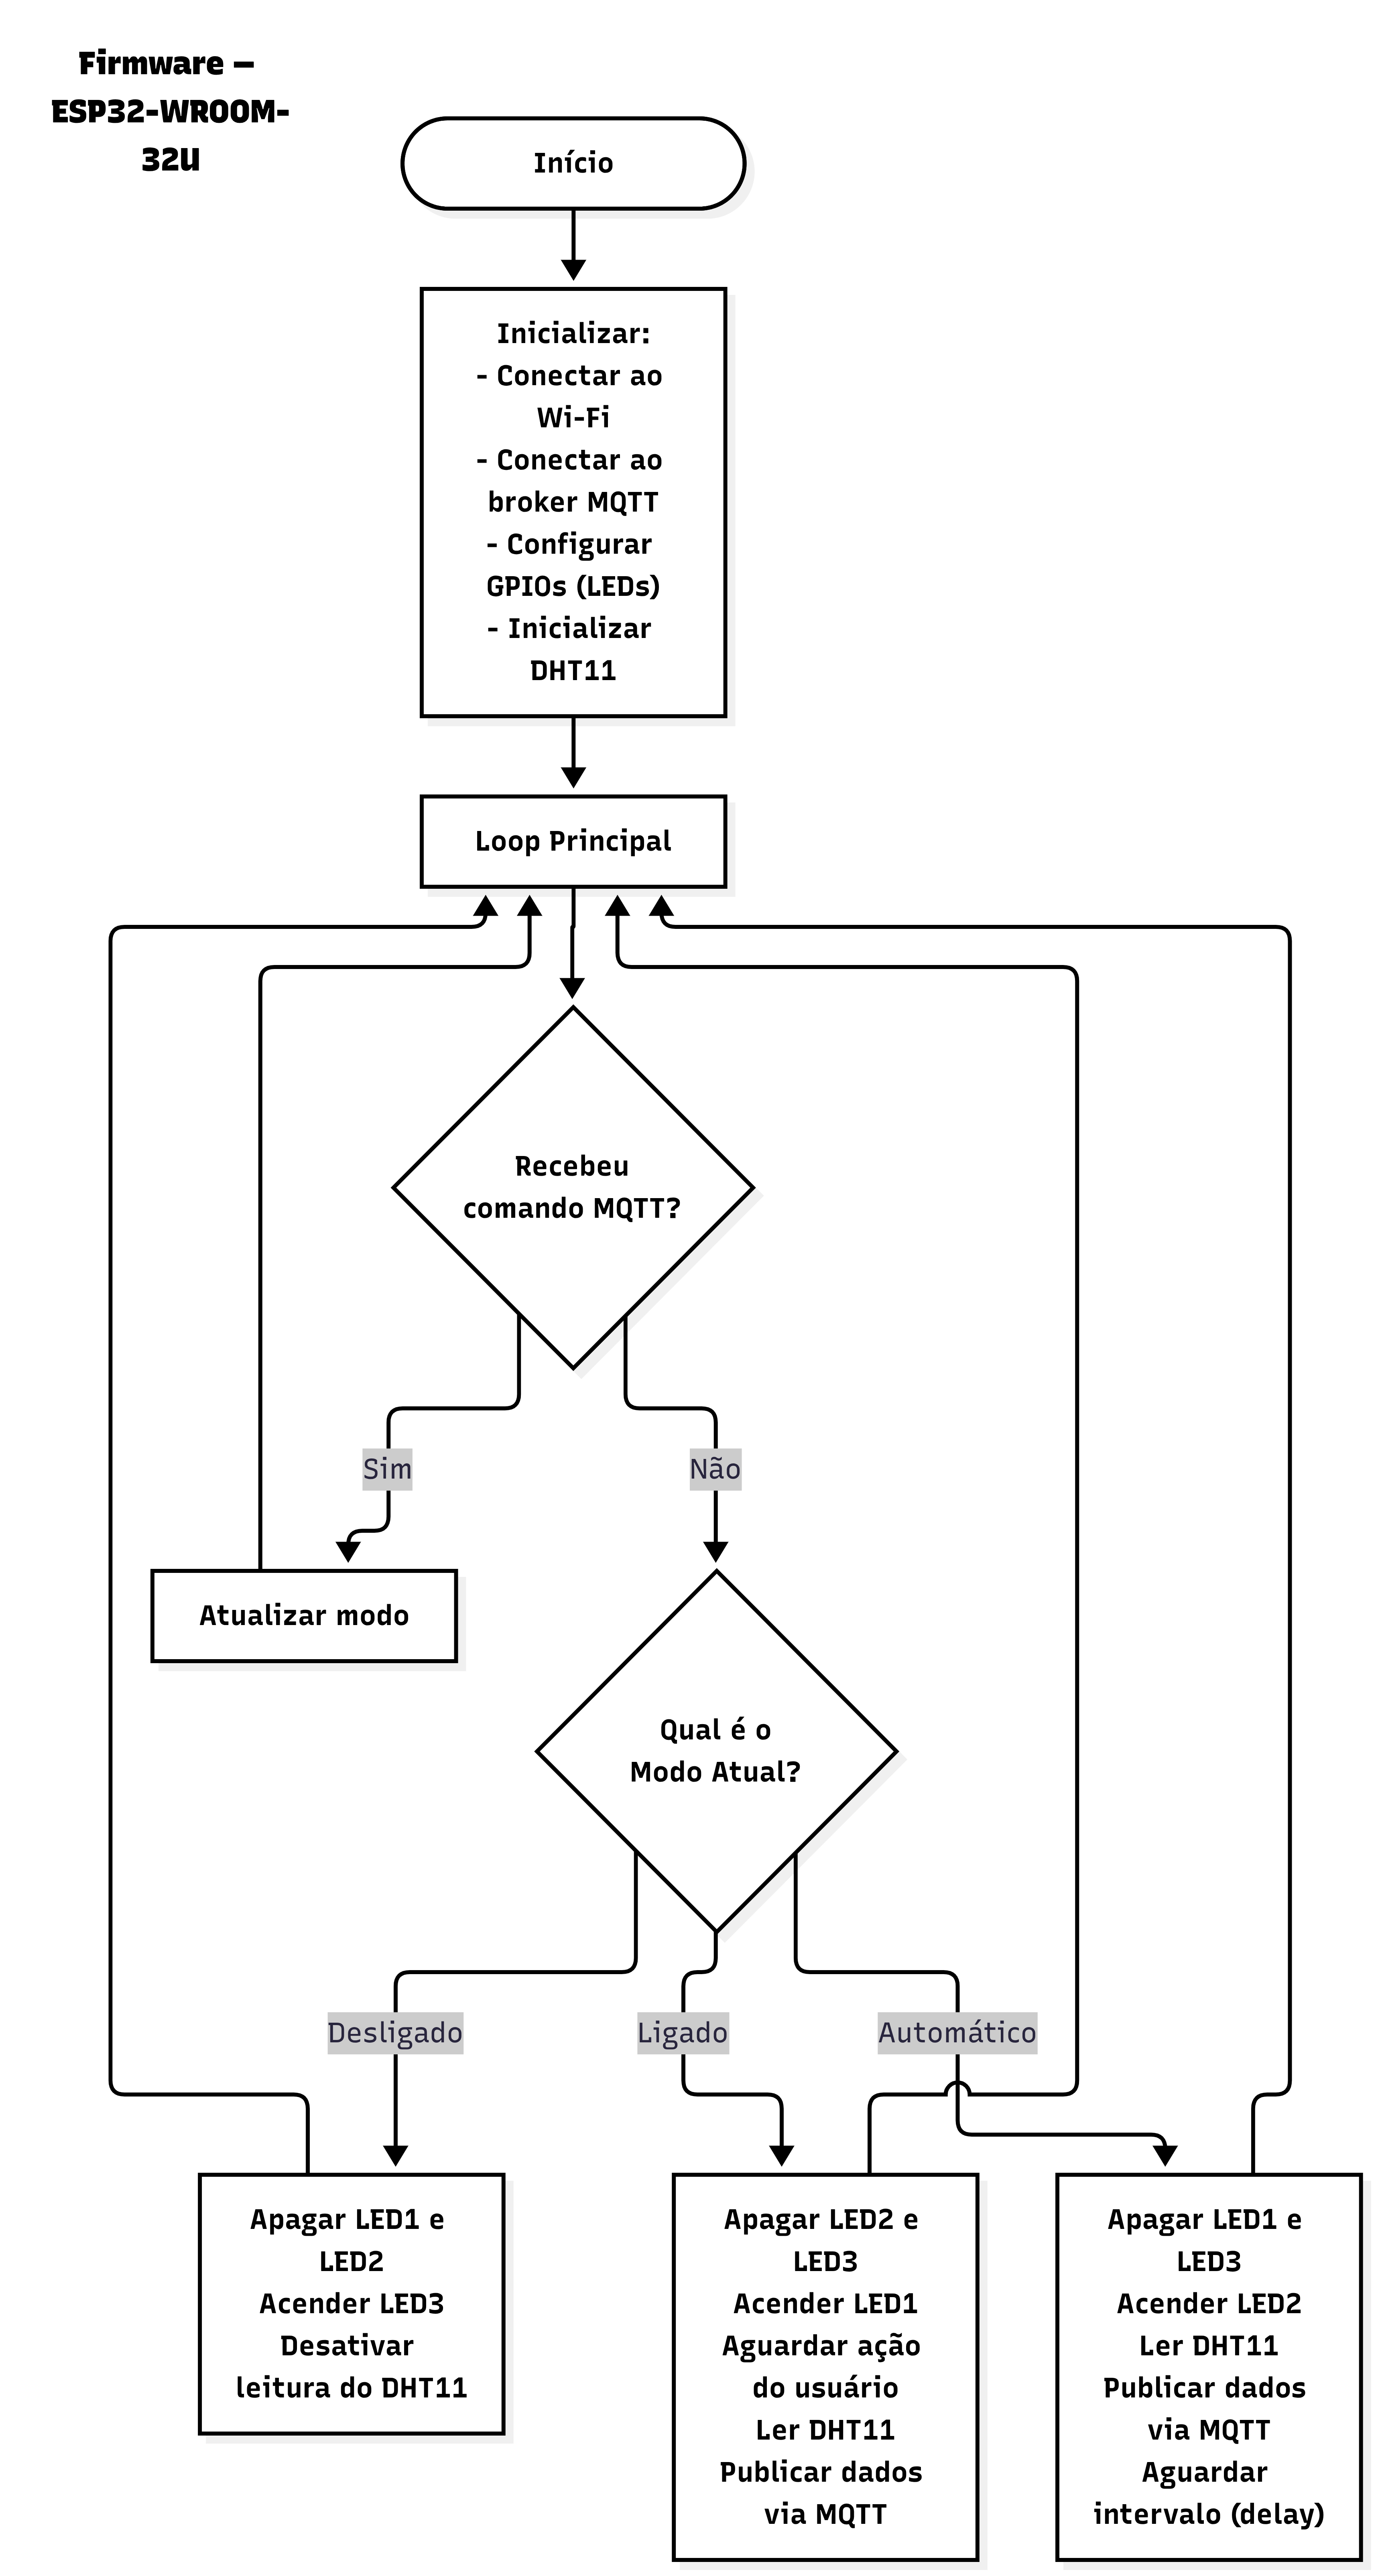
\includegraphics[width=\textwidth, height=0.78\textheight, keepaspectratio]{imag/diagrama-firmware.png}
    \caption{Diagrama de fluxo do firmware embarcado no ESP32.}
    \label{fig:diagrama-firmware}
\end{figure}

\subsubsection{Interface Web}

A interface web é servida pela API e acessada pelo usuário via navegador. Suas
funcionalidades na parte integral são:

\begin{itemize}
    \item \textbf{Exibição em tempo real:} Os dados de temperatura e umidade são
    atualizados dinamicamente na página via WebSocket ou polling da API, sem
    necessidade de recarregar a página.

    \item \textbf{Controle de modos:} A interface disponibiliza botões para
    alternância entre os modos Desligado, Ligado e Automático. Ao acionar um
    botão, a API publica o comando no broker MQTT, que é recebido pelo ESP32.

    \item \textbf{Indicação de modo ativo:} A interface exibe visualmente qual
    modo está ativo no momento, refletindo o estado do hardware.

    \item \textbf{Histórico de leituras:} A interface exibe uma tabela ou gráfico
    com o histórico das medições realizadas na sessão, incluindo data e hora de
    cada leitura.

    \item \textbf{Alertas automáticos:} Quando os valores de temperatura ou umidade
    ultrapassarem limites pré-definidos, a interface exibe um alerta visual
    destacado ao usuário.
\end{itemize}

\subsubsection{Protótipo de Baixa Fidelidade}

A Figura~\ref{fig:prototipo-baixa-fidelidade} ilustra o protótipo de baixa fidelidade
da interface, desenvolvido para validar a disposição estrutural dos elementos essenciais
do escopo obrigatório de entrega (apresentação dos dados de temperatura e umidade,
seleção e feedback de estado entre os modos Desligado, Ligado e Automático).

Ressalta-se que este modelo contempla estritamente as funcionalidades da parte integral.
Caso as funcionalidades da parte extra (como parametrização dinâmica de limites e gestão
de destinatários de e-mail) sejam consolidadas, o protótipo de interface será atualizado
em versões futuras da documentação.

\begin{figure}[H]
    \centering
    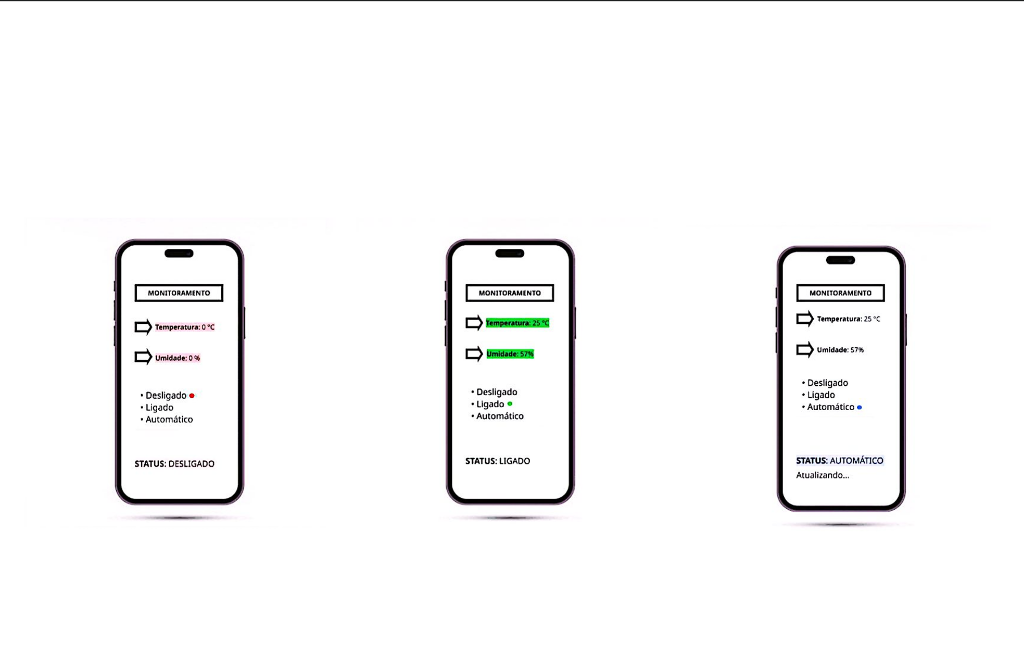
\includegraphics[width=\textwidth, height=0.45\textheight, keepaspectratio]{imag/prototipo-baixa-fidelidade.png}
    \caption{Protótipo de baixa fidelidade da interface nos modos Desligado, Ligado e Automático.}
    \label{fig:prototipo-baixa-fidelidade}
\end{figure}


% ====================================================================
\subsection{Parte Extra}
% ====================================================================
% Funcionalidades adicionais implementadas além do escopo mínimo.

\subsubsection{Log Local}

O sistema implementa persistência de dados por meio de um \textbf{log local em
arquivo \texttt{.txt}}. A cada leitura realizada pelo ESP32, a API registra um
entrada no arquivo de log contendo data, hora, temperatura e umidade. Esse
arquivo pode ser consultado ou exportado pelo usuário, garantindo histórico
persistente mesmo após reinicializações do sistema.

\subsubsection{Disparo de E-mail}

Quando os valores de temperatura ou umidade ultrapassarem limites configuráveis,
o sistema envia automaticamente uma \textbf{notificação por e-mail} ao usuário,
além do alerta exibido na interface web. O envio é realizado pela API via
protocolo SMTP, utilizando as credenciais e limites definidos nas configurações
do sistema.
